\documentclass{article}
% ===================================IEEE==================================
\usepackage{graphicx,amsmath,amssymb,url}      % include this line if your document contains figures
\usepackage[utf8]{inputenc}
\usepackage{float}
\usepackage[left=2cm,top=2cm,right=2cm,bottom=2cm]{geometry}


\usepackage{listings}
\usepackage{color}

\definecolor{dkgreen}{rgb}{0,0.6,0}
\definecolor{gray}{rgb}{0.5,0.5,0.5}
\definecolor{mauve}{rgb}{0.58,0,0.82}

\lstset{frame=tb,
  language=Matlab,
  aboveskip=3mm,
  belowskip=3mm,
  showstringspaces=false,
  columns=flexible,
  basicstyle={\small\ttfamily},
  numbers=none,
  numberstyle=\tiny\color{gray},
  keywordstyle=\color{blue},
  commentstyle=\color{dkgreen},
  stringstyle=\color{mauve},
  breaklines=true,
  breakatwhitespace=true,
  tabsize=3
}



\begin{document}

    \center
    {\huge Atividade Avaliativa - Física de Reatores }
    
    {Thalles Oliveira Campagnani}

    \raggedright
    \section{Exercício 1}

        \subsection{Enunciado}
            \begin{figure}[ht]
                \centering
                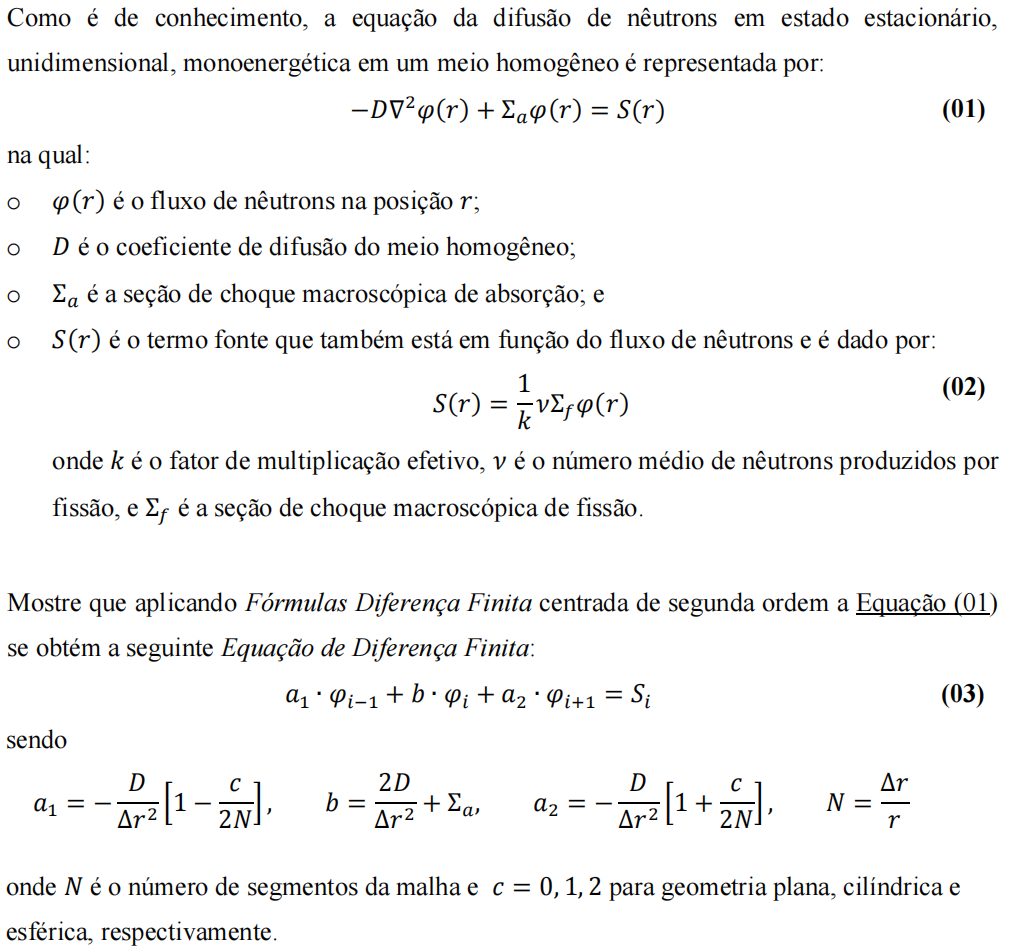
\includegraphics[width=15cm]{enun1.png}
                \centering 
                %\caption{Design hipotético de implementação de controlador PID para o \textit{NucleLink}. \centering }
                \label{nuclelink_fechado}
            \end{figure}
        \subsection{Dados}

            Equação da Difusão:
        
            \begin{equation}
                -D \triangledown^2 \phi (r) + \Sigma_a \phi(r) = S(r)
            \end{equation}
    
            tal que
    
            \begin{equation}
                S(r) = \frac{1}{k} v \Sigma_f \phi(r)
            \end{equation}

            Formulas de diferença:
        
            \begin{equation}
                f_{x|i} = \frac{f_{i+1} - f_{i-1}}{2 \Delta x} 
            \end{equation}
            
            e
            
            \begin{equation}
                f_{xx|i} = \frac{f_{i+1} - 2 f_i + f_{i-1}}{\Delta x^2} 
            \end{equation}

            Laplaciano para o caso unidimensional de coordenadas cartesianas:

            \begin{equation}
                \triangledown =  \frac{\partial^2}{\partial x^2} 
            \end{equation}
            
            Laplaciano para o caso unidimensional de coordenadas cilíndricas:
        
            \begin{equation}
                \triangledown =  \frac{\partial^2}{\partial r^2}  + \frac{2}{r} \frac{\partial}{\partial r}
            \end{equation}
           
            Laplaciano para o caso unidimensional de coordenadas esféricas:

            \begin{equation}
                \triangledown =  \frac{\partial^2}{\partial r^2}  + \frac{1}{r} \frac{\partial}{\partial r}
            \end{equation}
            
        \subsection{Desenvolvimento}

            \subsubsection{Plano}
    
                Aplicando o laplaciano para o caso caso cartesiano na equação da difusão e omitindo que os termos estão em função de x, temos que
                
                \begin{equation}
                    -D \frac{\partial^2\phi}{\partial x^2} + \Sigma_a \phi = S
                \end{equation}
        
                aplicando as formulas da diferença
        
                \begin{equation}
                    -D ( \frac{\phi_{i+1} - 2\phi_i + \phi_{i-1}}{\Delta x^2}  ) + \Sigma_a \phi_i = S_i
                \end{equation}
    
                colocando cada $\phi$ em evidência
                
                \begin{equation}
                    ( -\frac{D}{\Delta x^2} ) \phi_{i+1}    +    (\frac{2D}{\Delta x^2} + \Sigma_a) \phi_i    +    (-\frac{D}{\Delta x^2} ) \phi_{i-1} = S_i
                \end{equation}
    
                temos que
                
                \begin{equation}
                    a_p \phi_{i-1}    +    b_p \phi_i    +    c_p \phi_{i+1} = S_i
                \end{equation}
        
                Tal que
        
                \begin{equation}
                    a_p = \frac{-D}{\Delta x^2} = \frac{-D}{\Delta x^2} ( 1 - \frac{c}{2N}) 
                \end{equation}
                
                e
        
                \begin{equation}
                    b_p = \frac{2D}{\Delta x^2} + \Sigma_a
                \end{equation}

                e

                \begin{equation}
                    c_p = \frac{-D}{\Delta x^2} = \frac{-D}{\Delta x^2} ( 1 + \frac{c}{2N}) 
                \end{equation}
                
                Portanto concluímos que $c=0$ para o caso plano.
                
            \subsubsection{Cilíndrico}
    
                Aplicando o laplaciano para o caso caso cilíndrico na equação da difusão e omitindo que os termos estão em função de r, temos que
                
                \begin{equation}
                    -D ( \frac{\partial^2\phi}{\partial r^2}  + \frac{2}{r} \frac{\partial\phi}{\partial r} ) + \Sigma_a \phi = S
                \end{equation}
        
                aplicando as formulas da diferença
        
                \begin{equation}
                    -D ( \frac{\phi_{i+1} - 2\phi_i + \phi_{i-1}}{\Delta r^2}   +   \frac{2}{r}  \frac{ \phi_{i+1} - \phi_{i-1}}{ 2 \Delta r} ) + \Sigma_a \phi_i = S_i
                \end{equation}
    
                colocando cada $\phi$ em evidência
                
                \begin{equation}
                    ( -\frac{D}{\Delta r^2} - \frac{D}{r \Delta r} ) \phi_{i+1}    +    (\frac{2D}{\Delta r^2} + \Sigma_a) \phi_i    +    (-\frac{D}{\Delta r^2} + \frac{D}{r \Delta r} ) \phi_{i-1} = S_i
                \end{equation}
    
                temos que
                
                \begin{equation}
                    a_c \phi_{i-1}    +    b_c \phi_i    +    c_c \phi_{i+1} = S_i
                \end{equation}
        
                Tal que
        
                \begin{equation}
                    a_c = \frac{-D}{\Delta r^2} (1 - \frac{\Delta r}{r}) = \frac{-D}{\Delta x^2} ( 1 - \frac{c}{2N}) 
                \end{equation}
                
                e
        
                \begin{equation}
                    b_c = \frac{2D}{\Delta r^2} + \Sigma_a
                \end{equation}
                
                e
        
                \begin{equation}
                    c_c = \frac{-D}{\Delta r^2} (1 + \frac{\Delta r}{r}) = \frac{-D}{\Delta x^2} ( 1 + \frac{c}{2N}) 
                \end{equation}
    
                Portanto concluímos que $c=2$ para o caso cilíndrico.
                
            \subsubsection{Esférico}

                Aplicando o laplaciano para o caso caso esférico na equação da difusão e omitindo que os termos estão em função de r, temos que
            
                \begin{equation}
                    -D ( \frac{\partial^2\phi}{\partial r^2}  + \frac{1}{r} \frac{\partial\phi}{\partial r} ) + \Sigma_a \phi = S
                \end{equation}
        
                aplicando as formulas da diferença
        
                \begin{equation}
                    -D ( \frac{\phi_{i+1} - 2\phi_i + \phi_{i-1}}{\Delta r^2}   +   \frac{1}{r}  \frac{ \phi_{i+1} - \phi_{i-1}}{ 2 \Delta r} ) + \Sigma_a \phi_i = S_i
                \end{equation}
    
                colocando cada $\phi$ em evidência
                
                \begin{equation}
                    ( -\frac{D}{\Delta r^2} - \frac{D}{2r \Delta r} ) \phi_{i+1}    +    (\frac{2D}{\Delta r^2} + \Sigma_a) \phi_i    +    (-\frac{D}{\Delta r^2} + \frac{D}{2r \Delta r} ) \phi_{i-1} = S_i
                \end{equation}
    
                temos que
                
                \begin{equation}
                    a_e \phi_{i-1}    +    b_e \phi_i    +    c_e \phi_{i+1} = S_i
                \end{equation}
        
                Tal que
        
                \begin{equation}
                    a_e = \frac{-D}{\Delta r^2} (1 - \frac{\Delta r}{2r}) = \frac{-D}{\Delta x^2} ( 1 - \frac{c}{2N}) 
                \end{equation}
                
                e
        
                \begin{equation}
                    b_e = \frac{2D}{\Delta r^2} + \Sigma_a
                \end{equation}
                
                e
        
                \begin{equation}
                    c_e = \frac{-D}{\Delta r^2} (1 + \frac{\Delta r}{2r}) = \frac{-D}{\Delta x^2} ( 1 + \frac{c}{2N}) 
                \end{equation}
    
                Portanto concluímos que $c=1$ para o caso esférico.
    
    
    
    
    
    
    
    \newpage
    \section{Exercício 2}

        \subsection{Enunciado}
            \begin{figure}[ht]
                \centering
                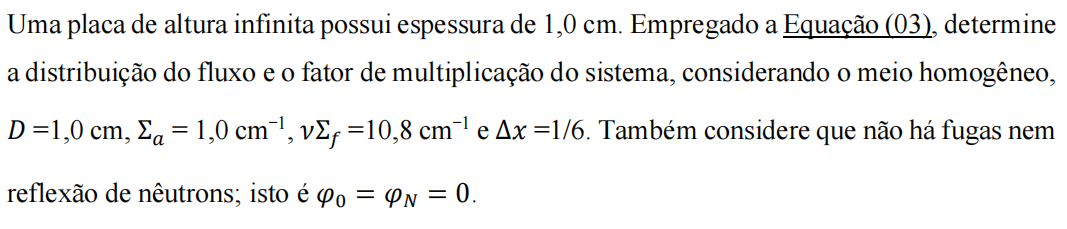
\includegraphics[width=15cm]{enun2.png}
                \centering 
                %\caption{Design hipotético de implementação de controlador PID para o \textit{NucleLink}. \centering }
                \label{nuclelink_fechado}
            \end{figure}

        \subsection{Desenvolvimento}

            \subsubsection{Analítico}

                Calculando $N$ temos que

                \begin{equation}
                    N = \frac{r}{\Delta r} = \frac{1}{\frac{1}{6}} = 6
                \end{equation}

                Iterando a equação (1) de $1$ até $N-1 = 5$, temos

                \begin{eqnarray}
                    i=1 \implies a_1 \phi_0 + b \phi_1 + a_2 \phi_2 = \frac{1}{k} S_1 \nonumber \\
                    i=2 \implies a_1 \phi_1 + b \phi_2 + a_2 \phi_3 = \frac{1}{k} S_2 \nonumber \\
                    i=3 \implies a_1 \phi_2 + b \phi_3 + a_2 \phi_4 = \frac{1}{k} S_3 \nonumber \\
                    i=4 \implies a_1 \phi_3 + b \phi_4 + a_2 \phi_5 = \frac{1}{k} S_4 \nonumber \\
                    i=5 \implies a_1 \phi_4 + b \phi_5 + a_2 \phi_6 = \frac{1}{k} S_5
                \end{eqnarray}

                pelas condições de contorno temos que

                \begin{equation}
                    \phi_0 = \phi_6 = 0
                \end{equation}

                logo

                \begin{eqnarray}
                    i=1 \implies b \phi_1 + a_2 \phi_2 = \frac{1}{k} S_1 \nonumber \\
                    i=2 \implies a_1 \phi_1 + b \phi_2 + a_2 \phi_3 = \frac{1}{k} S_2 \nonumber \\
                    i=3 \implies a_1 \phi_2 + b \phi_3 + a_2 \phi_4 = \frac{1}{k} S_3 \nonumber \\
                    i=4 \implies a_1 \phi_3 + b \phi_4 + a_2 \phi_5 = \frac{1}{k} S_4 \nonumber \\
                    i=5 \implies a_1 \phi_4 + b \phi_5 = \frac{1}{k} S_5
                \end{eqnarray}

                Podemos definir

                \begin{equation}
                    \Phi^T = [ \phi_1,\phi_2,\phi_3,\phi_4,\phi_5]
                \end{equation}

                e

                \begin{equation}
                    \textbf{S}^T = [ S_1,S_2,S_3,S_4,S_5]
                \end{equation}

                e

                \begin{displaymath}
                    \mathbf{\textbf{M}}=\left(\begin{array}{ccccc}
                    b   & a_2 & 0   & 0   & 0   \\
                    a_1 & b   & a_2 & 0   & 0   \\
                    0   & a_1 & b   & a_2 & 0   \\
                    0   & 0   & a_1 & b   & a_2 \\
                    0   & 0   & 0   & a_1 & b
                    \end{array}\right)
                \end{displaymath}

                Logo o sistema de equações pode ser escrito como a seguinte equação matricial

                \begin{equation}
                    \textbf{M}\Phi = \frac{1}{k}\textbf{S} 
                \end{equation}
                
                
            \subsubsection{Computacional}
            
                A partir do fluxograma abaixo, do dados do enunciado e dos cálculos algébricos que foram realizados, foi desenvolvido um algorítimo para resolver o problema
                \begin{figure}[H]
                    \centering
                    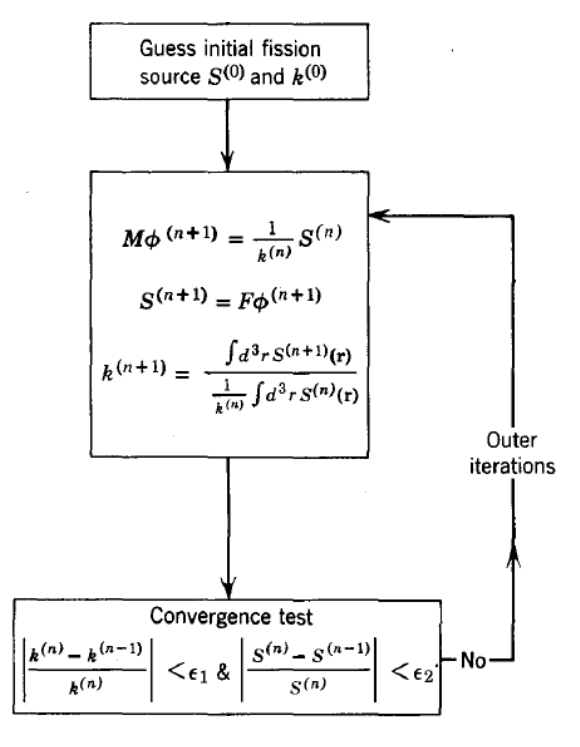
\includegraphics[width=8cm]{fluxograma.png}
                    \centering 
                    %\caption{Design hipotético de implementação de controlador PID para o \textit{NucleLink}. \centering }
                    \label{nuclelink_fechado}
                \end{figure}
            
                Código desenvolvido em linguagem MATLAB
                \begin{lstlisting}
clear
clc

%Dados
D        =  1.0;   %cm
Sigma_a  =  1.0;   %cm–1
vSigma_f =  10.8;  %cm–1
x        =  1;     %cm
dx       =  1/6;   %cm

%Formulas
N        =  x/dx;
a1       = -D/dx^2;
a2       = a1;
b        = 2*D/dx^2 + Sigma_a;

%Matriz
M = [
      b  a2   0   0   0;
     a1   b  a2   0   0;
      0  a1   b  a2   0;
      0   0  a1   b  a2;
      0   0   0  a1   b;
      ];
%Inversa da matriz
inv_M = inv(M);


% Chute inicial
k=1;
S = [
    1;
    1;
    1;
    1;
    1;
    ];


%Calculo de Phi a partir do chute inicial
phi = inv_M * S / k;

%Dados para loop
i   = 1;     %Variavel auxiliar 1
e   = 2;     %Variavel auxiliar 2
err = 0.001; %Erro máximo (criterio de parada)

%loop
while 1
    i = i + 1; %Primeiro phi já foi calculado, loop começa na segunda interação

    S(:,i) = vSigma_f * phi(:,i-1); %Calcule S
    
    k(i) = k(i-1) * ( S(1,i) + S(2,i) + S(3,i) + S(4,i) + S(5,i) ) / ( S(1,i-1) + S(2,i-1) + S(3,i-1) + S(4,i-1) + S(5,i-1) ); %Calcule K
    
    phi(:,i) = inv_M * S(:,i-1) / k(i-1); %Calcule phi
    
    %Condição de parada
    if (i>2 &&  (  abs(k(i) - k(i-e)) < err  )  &&  (  abs(S(1,i) - S(1,i-e)) < err  )  &&  (  abs(S(2,i) - S(2,i-e)) < err  )  &&  (  abs(S(3,i) - S(3,i-e)) < err  ))
        break;
    end
end
                \end{lstlisting}

            \subsubsection{Resultado}

                Executando o loop até que o erro entre uma iteração e outra seja de no máximo $1$ centésimo, resultou em um total de 9 interações.

                Os valores de $k$ para cada iteração podem ser vistos na tabela abaixo, o qual $i=1$ é o chute inicial.
                \begin{table}[H]
                    \begin{tabular}{|l|l|l|l|l|l|l|l|l|l|l|}
                    \hline
                    k_i & i=1    & i=2    & i=3    & i=4    & i=5    & i=6    & i=7    & i=8    & i=9    & i=10   \\ \hline
                    k   & 1.0000 & 0.9522 & 0.9522 & 1.0051 & 1.0051 & 1.0131 & 1.0131 & 1.0143 & 1.0143 & 1.0144 \\ \hline
                    \end{tabular}
                \end{table}
                
                Os valores de $\Phi$ para cada iteração podem ser vistos na tabela abaixo, o qual $i=1$ é o resultado do chute inicial.
                \begin{table}[H]
                    \begin{tabular}{|l|l|l|l|l|l|l|l|l|l|l|}
                    \hline
                    \Phi_i & i=1    & i=2    & i=3    & i=4    & i=5    & i=6    & i=7    & i=8    & i=9    & i=10   \\ \hline
                    \phi_1 & 0.0633 & 0.0633 & 0.0630 & 0.0630 & 0.0629 & 0.0629 & 0.0629 & 0.0629 & 0.0629 & 0.0629 \\ \hline
                    \phi_2 & 0.1006 & 0.1006 & 0.1078 & 0.1078 & 0.1088 & 0.1088 & 0.1090 & 0.1090 & 0.1090 & 0.1090 \\ \hline
                    \phi_3 & 0.1129 & 0.1129 & 0.1238 & 0.1238 & 0.1255 & 0.1255 & 0.1258 & 0.1258 & 0.1258 & 0.1258 \\ \hline
                    \phi_4 & 0.1006 & 0.1006 & 0.1078 & 0.1078 & 0.1088 & 0.1088 & 0.1090 & 0.1090 & 0.1090 & 0.1090 \\ \hline
                    \phi_5 & 0.0633 & 0.0633 & 0.0630 & 0.0630 & 0.0629 & 0.0629 & 0.0629 & 0.0629 & 0.0629 & 0.0629 \\ \hline
                    \end{tabular}
                \end{table}











    \newpage
    \section{Exercício 3}

        \subsection{Enunciado}
            \begin{figure}[ht]
                \centering
                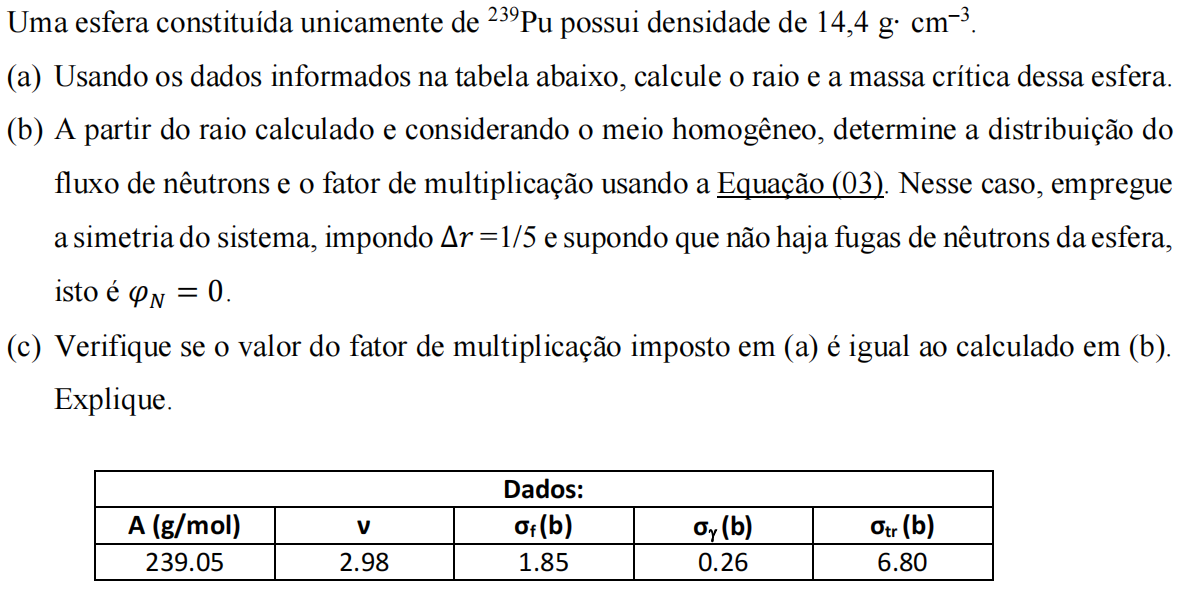
\includegraphics[width=15cm]{enun3.png}
                \centering 
                %\caption{Design hipotético de implementação de controlador PID para o \textit{NucleLink}. \centering }
                \label{nuclelink_fechado}
            \end{figure}

        \subsection{Desenvolvimento Letra A}

            Considerando a teoria da difusão para um único grupo de energia, temos que
            
            \begin{equation}
                k = \frac{v \frac{\Sigma_f}{\Sigma_a}}{1 + L^2 B_g^2}
                \label{eq_k}
            \end{equation}

            podemos considerar também as seguintes relações
            
            \begin{equation}
                 L^2 = \frac{D}{\Sigma_a}; ~~~~~~
                 D = \frac{1}{3\Sigma_{tr}}; ~~~~~~
                 B_g^2 = (\frac{\pi^2}{R})^2
                 \label{eq_relações}
            \end{equation}

            dado que estamos querendo encontrar o raio que torna a esfera crítica, podemos substituir $k=1$ na Eq. \ref{eq_k} e as relações da Eq. \ref{eq_relações} a fim de encontrar o raio $R$
    
            \begin{equation}
                \frac{v \frac{\Sigma_f}{\Sigma_a}}{1 + \frac{1}{3\Sigma_{tr}\Sigma_a} \frac{\pi^2}{\~{R}^2} } = 1
            \end{equation}

            realizando algumas álgebras em prol de isolar $\~{R}$
            
            \begin{equation}
                v \frac{\Sigma_f}{\Sigma_a} = 1 + \frac{1}{3\Sigma_{tr}\Sigma_a} \frac{\pi^2}{\~{R}^2}
            \end{equation}
    
            \begin{equation}
                v \frac{\Sigma_f}{\Sigma_a} - 1 = \frac{1}{3\Sigma_{tr}\Sigma_a} \frac{\pi^2}{\~{R}^2}
            \end{equation}
    
            \begin{equation}
                3\Sigma_{tr}\Sigma_a \~{R}^2 = \frac{\pi^2}{v \frac{\Sigma_f}{\Sigma_a} - 1}
            \end{equation}
    
            \begin{equation}
                \~{R}^2 = \frac{\pi^2}{ 3\Sigma_{tr}\Sigma_a (v \frac{\Sigma_f}{\Sigma_a} - 1)} = \frac{\pi^2}{ 3\Sigma_{tr} (v \Sigma_f - \Sigma_a)}
            \end{equation}

            chegamos a
            \begin{equation}
                \~{R} = \frac{\pi}{\sqrt{3}} \sqrt{\frac{1}{\Sigma_{tr} (v \Sigma_f - \Sigma_a)}}
            \end{equation}
    
            Podemos também considerar a relação entre seção de choque macroscópica e microscópica
            
            \begin{equation}
                \Sigma_i = N \sigma_i
            \end{equation}
            
            como a esfera é constituída unicamente de um material, temos que
    
            \begin{equation}
                \~{R} = \frac{\pi}{\sqrt{3}} \frac{1}{\sqrt{N\sigma_{tr} (v N\sigma_f - N\sigma_a)}} = \frac{\pi}{\sqrt{3}} \frac{1}{N\sqrt{\sigma_{tr} (v \sigma_f - \sigma_a)}}
            \end{equation}

            considerando a relação entre $\~{R}$ e $R$
            
            \begin{equation}
                \~{R} = R + a ; ~~~
                a = 0,71\lambda_{tr} ; ~~~
                \lambda_{tr} = \frac{1}{\Sigma_{tr}} ~~~
                \implies ~~~
                R = \~{R} - \frac{0,71}{N\sigma_{tr}} 
            \end{equation}

            temos que
            
            \begin{equation}
                R = \frac{\pi}{\sqrt{3}} \frac{1}{N\sqrt{\sigma_{tr} (v \sigma_f - \sigma_a)}} - \frac{0,71}{N\sigma_{tr}}
            \end{equation}

            Considerando que

            \begin{equation}
                N = \frac{\rho N_a}{M}
            \end{equation}

            e

            \begin{equation}
                \sigma_a = \sigma_f + \sigma_\gamma
            \end{equation}

            Calculando $R$ com os dados oferecidos na tabela, temos que

            \begin{equation}
                R = \frac{\pi}{\sqrt{3}} \frac{1}{\frac{14,4*6,022*10^{23}}{239,05}\sqrt{6,8*10^{-24} (2,98*1,85*10^{-24} - (0,26+1,85)*10^{-24})}} - \frac{0,71}{\frac{14,4*6,022*10^{23}}{239,05} 6,8*10^{-24}}
            \end{equation}

            logo

            \begin{eqnarray}
                R = 7,5159 cm \nonumber \\ %R = pi/sqrt(3) *  1/( (14.4*6.022*10^23/239.05) * sqrt(6.8*10^-24*(2.98*1.85*10^-24 - (0.26+1.85)*10^-24)))  - 0.71/((14.4*6.022*10^23/239.05)*6.8*10^-24)
                \~{R} = 10,3942 cm           %R = pi/sqrt(3) *  1/( (14.4*6.022*10^23/239.05) * sqrt(6.8*10^-24*(2.98*1.85*10^-24 - (0.26+1.85)*10^-24)))
            \end{eqnarray}

        \subsection{Desenvolvimento Letra B}

            \subsubsection{Analítico}

                Iterando a equação (1) de $0$ até $N-1 = 4$, temos

                \begin{eqnarray}
                    i=0 \implies a_1 \phi_{-1} + b \phi_0 + a_2 \phi_1 = \frac{1}{k} S_0 \nonumber \\
                    i=1 \implies a_1 \phi_0 + b \phi_1 + a_2 \phi_2 = \frac{1}{k} S_1 \nonumber \\
                    i=2 \implies a_1 \phi_1 + b \phi_2 + a_2 \phi_3 = \frac{1}{k} S_2 \nonumber \\
                    i=3 \implies a_1 \phi_2 + b \phi_3 + a_2 \phi_4 = \frac{1}{k} S_3 \nonumber \\
                    i=4 \implies a_1 \phi_3 + b \phi_4 + a_2 \phi_5 = \frac{1}{k} S_4 \nonumber
                \end{eqnarray}

                pelas condições de contorno temos que

                \begin{equation}
                    \phi_5 = 0
                \end{equation}

                e

                \begin{equation}
                    \phi_{-1} = \phi_1
                \end{equation}

                logo

                \begin{eqnarray}
                    i=0 \implies b \phi_0 + (a_1 + a_2) \phi_1 = \frac{1}{k} S_0 \nonumber \\
                    i=1 \implies a_1 \phi_0 + b \phi_1 + a_2 \phi_2 = \frac{1}{k} S_1 \nonumber \\
                    i=2 \implies a_1 \phi_1 + b \phi_2 + a_2 \phi_3 = \frac{1}{k} S_2 \nonumber \\
                    i=3 \implies a_1 \phi_2 + b \phi_3 + a_2 \phi_4 = \frac{1}{k} S_3 \nonumber \\
                    i=4 \implies a_1 \phi_3 + b \phi_4 = \frac{1}{k} S_4 \nonumber
                \end{eqnarray}

                Podemos definir

                \begin{equation}
                    \Phi^T = [ \phi_0,\phi_1,\phi_2,\phi_3,\phi_4]
                \end{equation}

                e

                \begin{equation}
                    \textbf{S}^T = [S_0,S_1,S_2,S_3,S_4]
                \end{equation}

                e

                \begin{displaymath}
                    \mathbf{\textbf{M}}=\left(\begin{array}{ccccc}
                    b   & a_1 + a_2 & 0   & 0   & 0   \\
                    a_1 & b   & a_2 & 0   & 0   \\
                    0   & a_1 & b   & a_2 & 0   \\
                    0   & 0   & a_1 & b   & a_2 \\
                    0   & 0   & 0   & a_1 & b
                    \end{array}\right)
                \end{displaymath}

                Logo o sistema de equações pode ser escrito como a seguinte equação matricial

                \begin{equation}
                    \textbf{M}\Phi = \frac{1}{k}\textbf{S} 
                \end{equation}

            \subsubsection{Computacional}
            
                A partir do fluxograma já citado, foi desenvolvido o seguinte código em linguagem MATLAB
                \begin{lstlisting}
clear
clc

%Dados
dens     = 14.4*6.022*10^23/239.05;  %densidade
D        = 1/(3*dens*6.8*10^-24);    %cm
Sigma_a  = dens*(0.26+1.85)*10^-24;  %cm–1
vSigma_f = 2.98*dens*1.85*10^-24;    %cm–1
r = 7.5159;%cm
N = 5;

%Formulas
dr = r/N;
a1 =  -D/dr^2 * (1 - 1/(2*N));
a2 =  -D/dr^2 * (1 + 1/(2*N));
b  = 2*D/dr^2 + Sigma_a;

%Matriz
M = [
      b  (a1+a2)    0   0   0;
     a1   b  a2   0   0;
      0  a1   b  a2   0;
      0   0  a1   b  a2;
      0   0   0  a1   b;
      ];
%Inversa da matriz
inv_M = inv(M);


% Chute inicial
k=1;
S = [
    1;
    1;
    1;
    1;
    1;
    ];


%Calculo de Phi a partir do chute inicial
phi = inv_M * S / k;

%Dados para loop
i   = 1;     %Variavel auxiliar 1
e   = 2;     %Variavel auxiliar 2
err = 0.005; %Erro máximo (criterio de parada)

%loop
while 1
    i = i + 1; %Primeiro phi já foi calculado, loop começa na segunda interação

    S(:,i) = vSigma_f * phi(:,i-1); %Calcule S
    
    k(i) = k(i-1) * ( S(1,i) + S(2,i) + S(3,i) + S(4,i) + S(5,i) ) / ( S(1,i-1) + S(2,i-1) + S(3,i-1) + S(4,i-1) + S(5,i-1) ); %Calcule K
    
    phi(:,i) = inv_M * S(:,i-1) / k(i-1); %Calcule phi
    
    %Condição de parada
    if (i>2 &&  (  abs(k(i) - k(i-e)) < err  )  &&  (  abs(S(1,i) - S(1,i-e)) < err  )  &&  (  abs(S(2,i) - S(2,i-e)) < err  )  &&  (  abs(S(3,i) - S(3,i-e)) < err  ))
        break;
    end
end
                \end{lstlisting}

            \subsubsection{Resultado}

                Executando o loop até que o erro entre uma iteração e outra seja de no máximo $5$ centésimos, resultou em um total de 9 interações.

                Os valores de $k$ para cada iteração podem ser vistos na tabela abaixo, o qual $i=1$ é o chute inicial.
                \begin{table}[H]
                    \begin{tabular}{|l|l|l|l|l|l|l|l|l|l|l|}
                    \hline
                    k_i & i=1    & i=2    & i=3    & i=4    & i=5    & i=6    & i=7    & i=8    & i=9    & i=10   \\ \hline
                    k   & 1.0000 & 1.2006 & 1.2006 & 1.2378 & 1.2378 & 1.2416 & 1.2416 & 1.2418 & 1.2418 & 1.2417 \\ \hline
                    \end{tabular}
                \end{table}
                
                Os valores de $\Phi$ para cada iteração podem ser vistos na tabela abaixo, o qual $i=1$ é o resultado do chute inicial.
                \begin{table}[H]
                    \begin{tabular}{|l|l|l|l|l|l|l|l|l|l|l|}
                    \hline
                    \Phi_i & i=1    & i=2    & i=3    & i=4    & i=5    & i=6    & i=7    & i=8    & i=9    & i=10   \\ \hline
                    \phi_1 & 7.8534 & 7.8534 & 8.7327 & 8.7327 & 8.9504 & 8.9504 & 9.0063 & 9.0063 & 9.0211 & 9.0211 \\ \hline
                    \phi_2 & 7.5200 & 7.5200 & 8.1978 & 8.1978 & 8.3436 & 8.3436 & 8.3773 & 8.3773 & 8.3857 & 8.3857 \\ \hline
                    \phi_3 & 6.6020 & 6.6020 & 6.8098 & 6.8098 & 6.8047 & 6.8047 & 6.7946 & 6.7946 & 6.7907 & 6.7907 \\ \hline
                    \phi_4 & 5.0989 & 5.0989 & 4.7948 & 4.7948 & 4.6648 & 4.6648 & 4.6241 & 4.6241 & 4.6124 & 4.6124 \\ \hline
                    \phi_5 & 2.9423 & 2.9423 & 2.4130 & 2.4130 & 2.2793 & 2.2793 & 2.2442 & 2.2442 & 2.2347 & 2.2347 \\ \hline
                    \end{tabular}
                \end{table}

            \subsection{Letra C}

            Não é igual. Valor de $k$ na letra 'A' é igual a $1$, enquanto foi encontrado na letra 'B' o valor de $k$ é igual a $1,2417$.

            Isso se deve ao fato que na letra 'A' foi considerada fuga de nêutrons, enquanto na letra 'B' foi considerada que a fuga é nula.
\end{document}

